\section{Testgetriebene Entwicklung}
\label{sec:tdd}
Testgetriebene Entwicklung, im Englischen Test-Driven-Development (TDD) wurde erstmalig von Kent Beck 2002 im Detail erläutert \citep{beck_test_2002}. Zuvor war die Technik "`Test-First"' aber schon seit 1999 im Kontext von Extreme Programming (XP) bekannt.

Test-Driven-Development wird als
$$ \text{TDD} := \text{Test-First} + \text{Refaktorisieren}$$
\borderquote{TDD is also good for geeks who form emotional attachments to code. }{\citeauthor{beck_test_2002}}
beschrieben \citep{scott_ambler_introduction_2002}. So ist es Ziel, dass sich Test schreiben/Implementation und Refaktorisierungen, d.h. das konstante Verbessern des Systemdesigns und des Quellcodes, abwechseln. Mittlerweile werden die Begriffe Test-First Development und \glossar{TDD} synonym verwendet, allerdings gibt es manchmal Unterschiede in der Herangehensweise in Punkto Design der Software: TDD findet seine Anwendung, wenn nur eine vage Idee der Funktionalität einer Klasse besteht, während TFD kein Design oder Redesign der Klassen vorsieht \citep{stackoverflow_testing_2008}.

% \paragraph{Einordnung} Da bei der Testgetriebenen Entwicklung die funktionalen Anforderungen der treibende Faktor für die Implementation der Tests sind, können die dabei entstehenden Testfälle den funktionalen Tests zugeordnet werden. In der Sichtbarkeit des Quellcodes sind die Tests der Testgetriebenen Entwicklung ein Spezialfall: Sie sind weder reine Whitebox-, nocht Blackboxtests, sondern Greyboxtests, da der zugrundeliegende Quellcode zwar (noch) nicht bekannt ist, aber 


Im Folgenden wird die Entwicklungsmethode \glossar{TDD} näher beleuchtet und am Beispiel von \glossar{rails} typische Testwerkzeuge aufzeigen. 
\subsection{Motivation}
  Das Erstellen einer gut-abdeckten \glossar{testsuite} für ein jedes größeres Softwareprojekt ist eine wichtige Voraussetzungen um interne Qualitäten, wie Wartbarkeit und Zuverlässigkeit zu aktivieren. \glossar{TDD} soll nicht dazu dienen, die Software zu auf Korrektheit zu untersuchen\footnote{TODO Kent Beck Verification und ISO 9000:2005 3.8.5}. Dies ist aber ein positiver Nebeneffekt. Das Hauptziel ist es, den Code in Einklang mit dem Test zu schreiben, so dass der Test den Code antreibt (Test drives the code). Der messbare Effekt davon, ist ein gut-testbarer Code, welcher in der Regel auch ein gut-wartbarer und verständlicher Code ist. \glossarpl{smell}, wie God-Methode und geringe Kohäsion, werden schon im Keim erstickt werden, da diese nur äußerst schwer zu testen sind.

  \paragraph{Psychologische Aspekte und Aspekte des Projektmanagements}
  
  Kent Beck beschreibt die Hauptmotivation für TDD, als das "`managing fear during programming"' Management von Angst. So hat Angst verschiedene Auswirkungen auf die Entwicklung. Sie mache zögerlich, führe zu weniger Kommunikation und Feedback und mache den Programmierer "`mürrisch"' \citep[S. xi]{beck_test_2002}.
  
  TDD fördert die Entwicklung in kleinen Schritten, und ermöglicht durch bestandene Tests kleine "`Belohnungen"' für den Programmierer. Dadurch ist es leichter einen gewissen Arbeitsrhythmus zu erhalten, was stellenweise dem "`Flow"'\footnote{Schaffen-, Tätigkeitssrausch}  ähnelt oder diesen strukturiert ergänzen kann \citep{roger_brown_test_2008}.
  %Die Motivation für die Wahl von Test-getriebener Entwicklung als primäre Entwicklungsstrategie wird mit dem
  
  Falls TDD die Fehlerdichte signifikant verringern würde und nur Code entstünde, der getestet wurde, so hätte dies wohl auch soziale Auswirkungen auf das Entwicklerteam \citep[S. x]{beck_test_2002}. 
  \begin{enumerate}
   \item Die Qualitätssicherung könnte von einer reaktiven, auf eine proaktive Arbeit umstellen.
   \item Der Projektmanager kann den Ablauf der Entwicklung besser planen, da weniger überraschende Regressionsfehler im Laufe der Entwicklung auftreten
   \item Durch eine niedrige Fehlerdichte kann die Kontinuierliche Integration (Continuos Integration) möglich gemacht werden, und so der Kunde in den Entwicklungsprozess einbezogen werden
  \end{enumerate}
 
  
  
\subsection{Ablauf}
  Ziel ist es, vor der Implementation eines Codes, einen Unittest zu implementieren. Davon ausgehend soll der geringstmögliche Code implementiert werden, damit der Test besteht. Alles Drittest folgt die Refaktorisierung, bei TDD als Designphase genutzt.
  
  \begin{figure}[htbp]
 \centering
 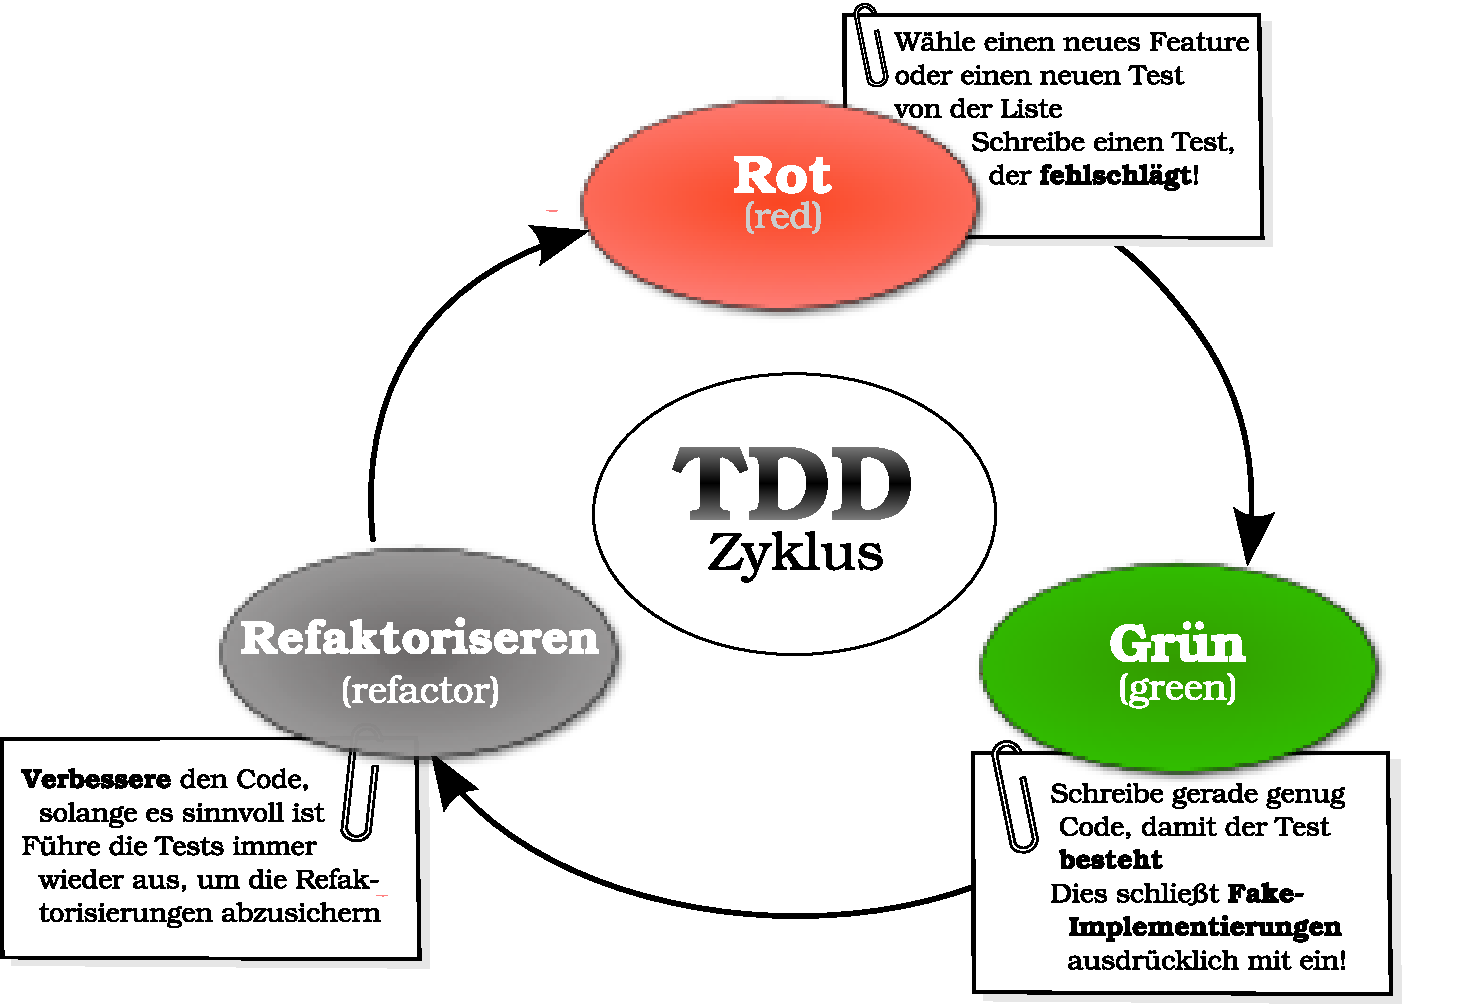
\includegraphics[width=0.85\textwidth]{./diagrams/red-green-refactor.pdf}
 % red-green-refactor.png: 884x602 pixel, 90dpi, 24.95x16.99 cm, bb=
 \caption{Red-Green-Refactor: Der TDD Entwicklungszyklus}
 
 \imgsource{Bildquelle: Der Autor}
 \label{fig:redgreenrefactor}
\end{figure}
  Im Detail sind das also folgende Phasen, vgl. Abbildung \ref{fig:redgreenrefactor}:
  \begin{enumerate}
   \item Schreibe einen neuen \glossar{test}. Dies kann der erste eines neuen Features sein, oder aber ein Test, um Funktionalität zum aktuellen Feature hinzuzufügen
   \item \textbf{Red}: Führe alle Tests aus, um sicherzugehen, dass der Test fehlschlägt. Andernfalls ist der Test überflüssig.
   \item \textbf{Green}: Nachdem der Test fehlschlägt, implementiere nun den einfachsten Code, damit der Test besteht\\
   Dies kann ausdrücklich auch eine Fake-Implementierung sein, also z.B. die Rückgabe eines konstanten Wertes anstelle einer Berechnung. Wichtig ist, dass diese Phase so schnell wie möglich verlassen wird.
   \item \textbf{Refactor}: Nachdem der Test bestanden wird, folgt nun die \textbf{wichtigste Phase}, die Refaktorisierungsphase.\\
   Da wir bereits einen Test haben, der unser gewünschtes Systemverhalten widerspiegelt, können wir gefahrlos \glossar{refaktorisieren}, d.h. meist Duplikation eliminieren. In dieser Phase findet das Design des Codes statt. Man macht sich Gedanken, wie die vorhanden Klassen optimal refaktorisiert werden können, um \glossarpl{smell} zu eliminieren, und welches Entwurfsmuster ggf. angewendet werden kann.
  \end{enumerate}
  
  
  Ein genau spezifizierter Ablauf ist in Abbildung \ref{fig:tddflow} zu finden. Auch dort ist zu sehen, dass die Testerstellungs und Refaktorisierungsphase strikt getrennt sind. Innerhalb ersterer solle nur möglichst schnell ein funktionierender Test erstellt und zum Bestehen gebracht werden. Die eigentliche Arbeit findet dann innerhalb der Refaktorisierungsphase statt, in der die wahrscheinlich suboptimale Implementierung verbessert wird, indem iterativ Design hinzugefügt wird.
  \begin{figure}[hp]
 \centering
 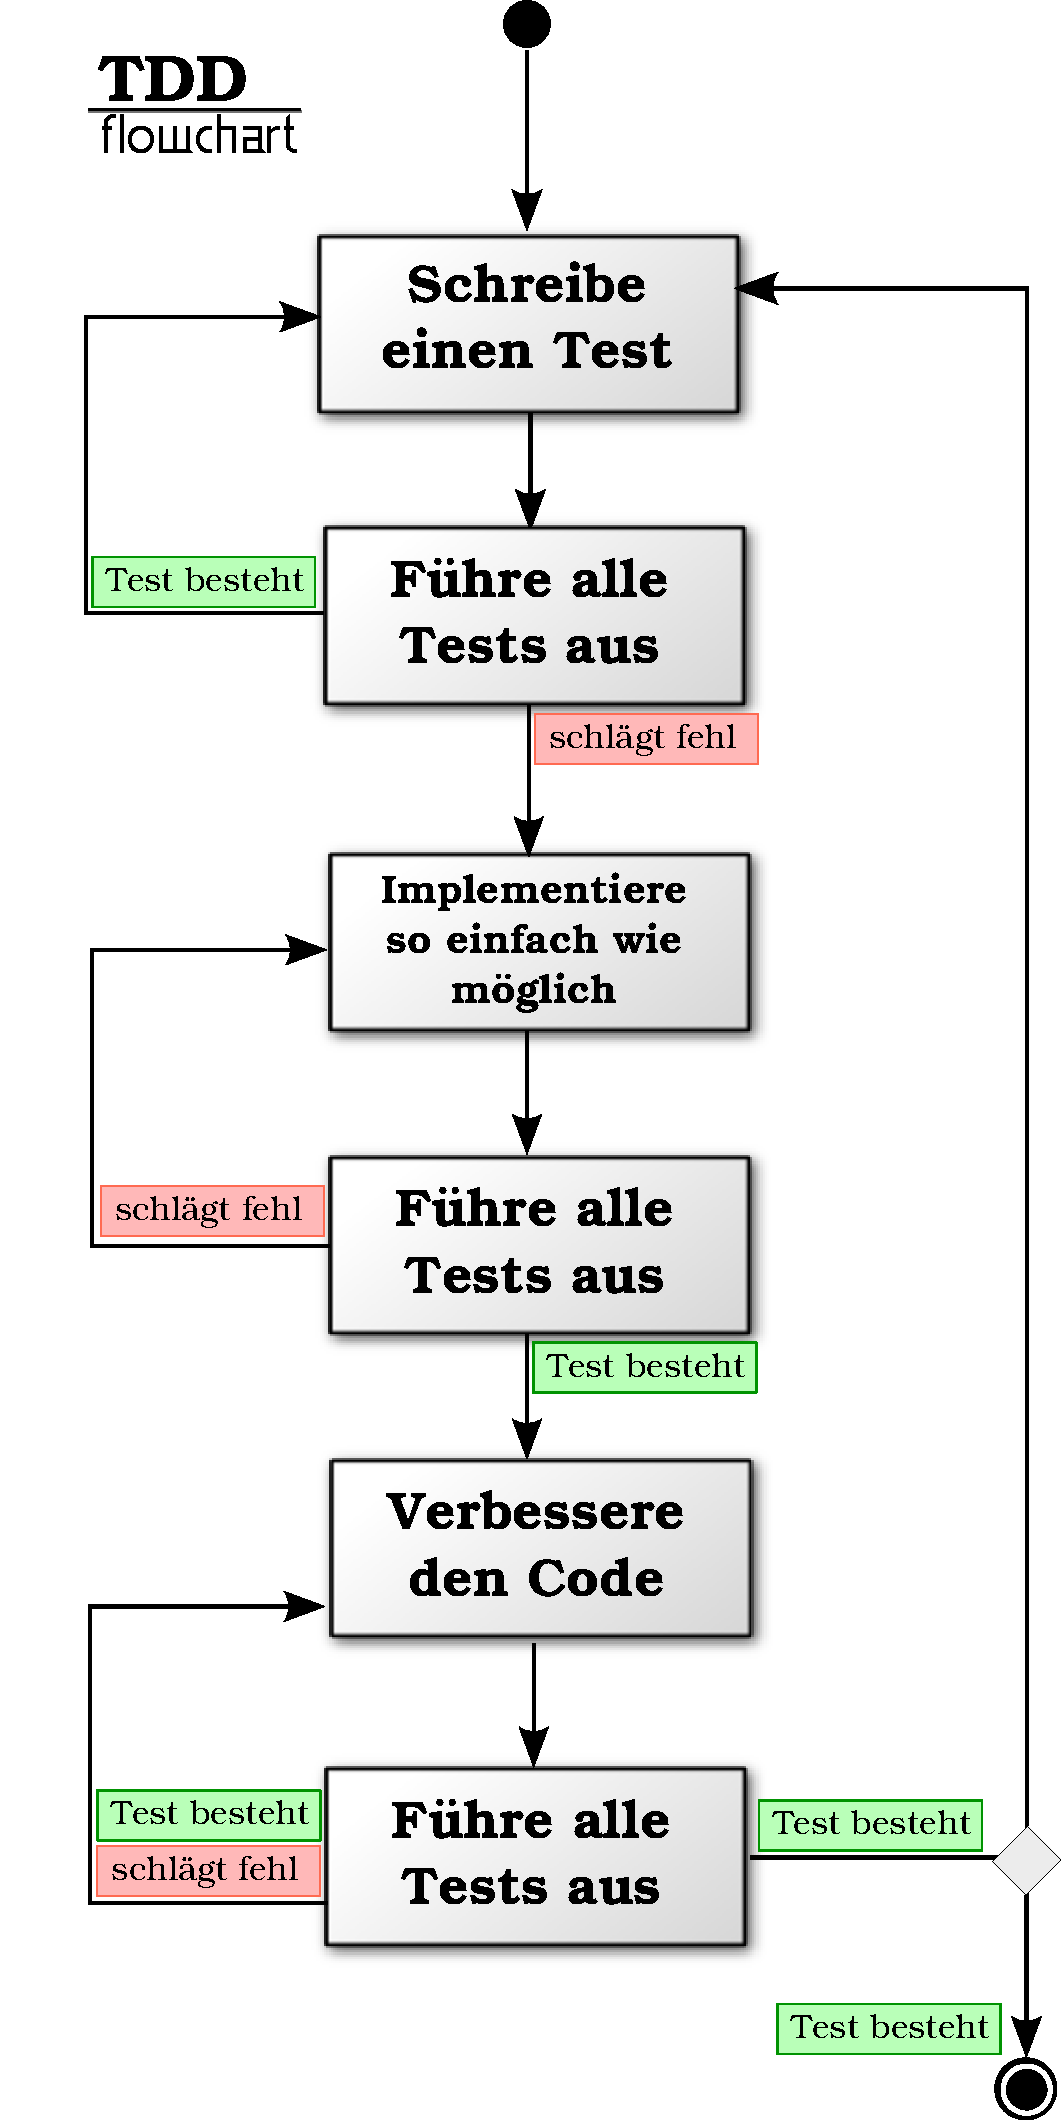
\includegraphics[width=0.75\textwidth]{./diagrams/tdd-flowchart.pdf}
 % tdd-flowchart.pdf: 510x1017 pixel, 72dpi, 17.99x35.88 cm, bb=0 0 510 1017
 \caption{Flussdiagram für TDD}
 \label{fig:tddflow}
 \imgsource{Bildquelle: Der Author}
\end{figure}


  Jeder Unittest soll prinzipiell nur eine Eigenschaft testen, die Entwicklung erfolgt also in kleinen Schritten. Dies hat direkte Auswirkungen auf die zu entwickelnden Objekte und Methoden, die ebenfalls übersichtlich werden sollen, und somit dem Objektbegriff, eine Klasse für eine Aufgabe, gerecht werden.
  
    \begin{figure}[hbtp]
 \centering
 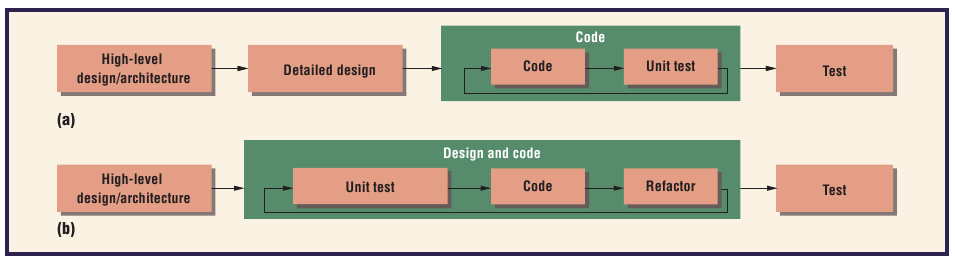
\includegraphics[width=\textwidth]{./diagrams/ablauf.png}
 % ablauf.png: 955x263 pixel, 96dpi, 25.26x6.96 cm, bb=0 0 716 197
 \caption{Entwicklungsablauf}
 \caption*{(a) Traditionelle Entwicklung,  b) Testgetriebene Entwicklung}
 \imgsource{Quelle: \citep{janzen_does_2008}}
 \label{fig:devflow}
\end{figure}
\borderquote{It's about the design, not the tests.}{Kent Beck}
  Aus der Sicht des gesamten Entwicklungsprozesses wird somit die klassische Design-Phase in die Implementation eingegliedert. In Abbildung \ref{fig:devflow} wird der klassische Entwickungsablauf dem Ablauf bei einem TDD-orientierten Ablauf verglichen. Demnach wird die (Fein-)Design Phase scheinbar aus dem Ablauf entfernt, und findet sich als Refaktorisierungsphase wieder. Wichtig zu bemerken ist außerdem, dass TDD keineswegs auf eine Analysephase/einen Grobentwurf oder finale (System)-Tests verzichtet, sondern nachwievor auf diese angewiesen ist. 
  


  
  \subsection{Sonderfälle}
  
  Der oben gezeigt Ablauf ist für den Normalfall, dem Entwickeln eines neuen Features gedacht. Für einige gesonderte Problemstellungen im Programmieralltag existieren ebenso gewisse Abläufe.
  
  \paragraph{Fehlerbehebung} Falls trotz der Verwendung von \glossar{TDD} Fehler in der Software gefunden werden, so erfolgt:
  \begin{enumerate}
   \item Schreibe einen Test, der den Fehler auslöst bzw. nachbildet
   \item Behebe den Fehler im Programmcode
   \item Führe alle Tests aus
  \end{enumerate}.
  Somit wird sichergestellt, das jeder bisher gefundene Fehler durch einen Test abgesichert wird.
  \paragraph{Spikes oder Spike Solution} In einigen Fällen ist es nicht ratsam, sofort mit einer testgetriebenen Entwicklung zu beginnen. Gerade wenn Prototypisierung, d.h. schnelle, erforschende, explorative Entwicklung mit dem ausschließlichen Ziel schnell ein lauffähiges Ergebnis zu erhalten, dann kann auf Tests verzichtet werden. Eine solches, isoliert entwickeltes Experiment wird im \glossar{TDD}-Jargon "`Spike"' (zu deutsch: Spitze, Nadel) genannt. Die Idee dahinter ist es zu Lernen, und der produzierte Code wird i.d.R. gelöscht und nach dem Lernprozess nach originärer TDD-Manier entwickelt. Dies soll auch die gewählte Metapher einer Nadel aufzeigen: Schnell eine Nadel durch ein Brett bringen \citep{shore_art_2007}. Ausführliche Informationen über das Wann und Wie eines Einsatzes von Spikes finden sie in dem Buch "`The Art of Agile Development"' \citep{shore_art_2007}. Der Autor hat sogar das betreffende Kapitel online verfügbar gemacht\footnote{\url{http://jamesshore.com/Agile-Book/spike_solutions.html}}.

  \paragraph{Testen von privaten Methoden und Variablen} Da die objektorienterte Modellierung das Konzept des Information Hiding und Kapselung vorsieht, soll der interne Aufbau einer Klasse nach außen nicht sichtbar sein. Da Tests aber von außen auf eine Klasse zugreifen, stellt dies ein Problem dar. In einigen Sprachen löst man sich dieses Problem mittels Reflections, um über Umwege auf private Felder zuzugreifen. Dies spielt allerdings nur für das nachträgliche Testen von Legacy-Anwendungen eine Rolle. TDD in der Reinform betrieben habe niemals spezfische Tests von privaten Methoden oder Feldern, da diese ausschließlich durch Refaktorisierung enstanden sein könnten \citep{caroli_agile_2008}.
 % http://agiletips.blogspot.com/2008/11/testing-private-methods-tdd-and-test.html 
 
  
  
  
  \subsection{ATDD -- Acceptance TDD}
  \label{sec:attd}
  Die Akzeptanztest-getriebene Entwicklung ist eine Modifikation von \glossar{TDD}. Statt der Unittests, stehen hier die Akzeptanztests im Vordergrund
  
  Das ganze lässt sich auch in den übergeordneten Prozess zum Entwickeln eines Features einordnen.
  %TODO RSPEC Buch macht das vor, Noch mal schauen, evtl alles Käse was ich hier geschrieben habe
  \begin{enumerate}
   \item Schreibe einen Akzeptanztest/Systemtest um das aktuelle Feature zu implementieren
   \item Implementiere die Teilschritte, die notwendig sind, um den Akzeptanztest bestehen zu lassen. Verfahre bei der Implementation nach dem TDD Schema zur Implementierung der benötigten Units wie oben.
    \begin{enumerate}
     \item Schreibe einen Unittest
     \item Prüfe, ob der Test fehlschlägt, andernfalls zurück zu 1.
     \item Implementiere mit so wenig wie möglich so, dass der Test besteht
     \item Refaktorisiere
    \end{enumerate}
   \item Nachdem der Akzeptanztest besteht, Prüfe etwaige Refaktorisierungen für die Anwendungsebene.   
  \end{enumerate}
  
  Somit werden 2 Testebenen erstellt, die Akzeptanz- und die Unittests.


\subsection{Prinzip des Emergent Design -- Evolutionäres Sofwaredesign}
Ein Konzept von TDD ist das, des sich Herausbildenden Designs. Gegenüber traditionellen Entwicklungsansätzen erfolgt die Entwicklungsphase (Design) nicht als eigenständige Phase, sondern ist streng in den Entwicklungsprozess integriert. Immer wenn ein Zyklus beim Refaktorisieren angelangt ist, findet effektiv Design statt. Eine Entwicklung nach TDD sucht den minimalsten Code, der die Anforderungen (Tests) erfüllt. Analog dazu, will ein Emergentes Design die kleinste Menge an benötigten Design suchen, im Gegensatz zu einem Software-Design, das im Vorfeld bedacht wurde. Durch die vielen Iterationen und die darausfolgenden zahlreichen Refaktorisierungen tritt nach und nach das Design hervor, welches optimal für das System ist. 



%discovering and harvesting patterns in existing Code

%GoF Patterns

%idiomatische Patterns: Patterns, die nur für genau eine Applikation oder innerhalb eines Unternehmens optimal sind. z.B. Security 
%technical patterns

%domain patterns -> common business patterns

%emergent -> discover this
%traditional design -> too early, Business Process can change way faster, speculation without facts
%Frameworks sollten nicht designt werden, sondern sich aus Code ergeben


%im Gegensatz zu einer Ingenieurswissenschaftlichen Tätigkeit, das ... -> Iterativ
% ward cummingham
%http://www.developerdotstar.com/mag/articles/reeves_design.html
%http://confreaks.net/videos/282-lsrc2010-real-software-engineering
%http://www.ibm.com/developerworks/java/library/j-eaed5/index.html

%because you think about every little component that goes into the system
%cheap to build, expensive to design
%BDUF (Big Design Upfront)


%http://www.thoughtworks.com/emergent-design

Einige Software-Architekten (\citeauthor*{neal_ford_emergent_2010}, \citeauthor*{jack_reeves_three_1992} und \citeauthor{glenn_vanderburg_real_2010}) proklamieren, dass praktisches Software-Engineering eigentlich keine ordinäre Ingenieursdisziplin sei. Ingenieure sind für die Planung und das Design verantwortlich, welches in aller Regel im Vorfeld der Implementierung stattfindet. Das klassische Software-Engineering empfindet diesen Prozess nach, was sich z.B. in dem Wasserfallmodell äußert. Diese Autoren äußern nun, dass dies für die meisten Softwareprojekte nicht ideal sei, da sich die Businessanforderungen meist im Laufe einer Entwicklung ändern. Traditionelles Softwaredesign abstrahiere zu früh und spekuliere ohne die letztendlichen Fakten zu kennen. Traditionelle Ingenieurswissenschaftliche Diszplinen haben außerdem die Beschränkung, dass ein Build-Prozess äußerst teuer ist (man denke an Brücken oder Chips in Flugzeugsystemen), wohingegen dies bei Software in der Regel fast nichts koste. Dadurch kann die Software-Entwicklung ein iteratives Vorgehen nutzen \citep{neal_ford_emergent_2010}, \citep{glenn_vanderburg_real_2010}, \citep{jack_reeves_three_1992}. Statt eines großen Designs am Anfang (BDUF -- Big Design Upfront) soll das Design durch Entdeckung und Extrahieren aus dem Sourcecode gewonnen werden.


Ein Emergent Design kann auch ohne TDD verwendet werden. Allerdings ist dies ohne das Vorhandensein von einer guten Test-Suite ein risikoreiches Unterfangen.
Mit seiner iterativen Herangehensweise passen Emergent Design in Kombination mit TDD dagegen perfekt in den Entwicklungszyklus der Agilen Software Entwicklung.


\subsection{Varianten}



  \subsubsection{Behavior Driven Development}
  
  Eine oft erwähnte Variante von TDD ist die Verhaltensgetriebene Entwicklung (Behavior-Driven-Development -- BDD). Dabei dienen hier Akzeptanztests als treibende Kraft der Entwicklung. Diese beschreiben ein Verhalten (Behavior). Der Fokus liegt also nicht auf Implementationsdetails, sondern soll, in einer domainspezifischen Sprache, das Verhalten und die daraus resultierenden Erwartungen des Systems beschreiben.
  
  Dies drückt sich meist auch in dem Vokabular aus. Während bei klassischen Unit-Tests, und damit auch bei TDD, die Begriffsdomain  "`Zusicherungen"' (assertions) und "`Tests"' beinhaltet, so hat BDD stattdessen "`Erwartungen"' (expectations) und "`Spezifikationen"' (specs/specifiations), und verwendet oft das Modalverb "`sollte"' (should).
  
  % TODO Beispiel
 \subsubsection{Design Driven Testing}
  Design Driven Testing soll eine Umkehrung von Testgetriebener Software sein und wird Stephens und Rosenberg als Alternative dazu vorgeschlagen \citep{stephens_design_2010}. Sie kritisieren, dass TDD in Reinform betrieben, lediglich Unittests, aber keine Dokumentation oder höhere Tests höherer Levels produziert. Weiterhin monieren sie, dass TDD zu schwierig und aufwändig sei. Sie schlagen vor, stattdessen die Tests durch das Software-Design steuern zu lassen und sich auf komplexe Code-Abschnitte zu konzentrieren, anstatt wirklich jeden Code durch einen vorausgegangen Test entstehen zu lassen. Sie proklamieren die Nutzung von Akzeptanz- anstelle der Unittests. Code-Qualität soll durch ein gründliches vorheriges Design anstelle nachträglicher massiver Refaktorisierungen bewerkstelligt werden.
  DDT eignet sich für größere Teams, da Wert auf manuelle Tests gelegt wird und z.B. ein QA-Team eingebunden wird. Da das Projektteam von it-jobs-und-stellen.de ein sehr kleines ist, wird auf diesen Entwicklungsprozess nicht näher eingegangen.